% !TeX root = RJwrapper.tex
\title{Capitalized Title Here}
\author{by Author One, Author Two}

\maketitle

\abstract{%
An abstract of less than 150 words.
}

\hypertarget{real-rata-and-simulations}{%
\subsection{Real Rata and Simulations}\label{real-rata-and-simulations}}

\hypertarget{boston-housing-data}{%
\subsubsection{Boston Housing data}\label{boston-housing-data}}

\begin{Schunk}
\begin{Sinput}
#source the functions. Will be changed to load package
source("../R/SINDEXQ_fun.R")

#load data from MASS
library(MASS)
#help(Boston)
medv<- Boston$medv
RM <- Boston$rm
logTAX <- log(Boston$tax)
PTRATIO <- Boston$ptratio
logLSTAT <- log(Boston$lstat)

X <- cbind(RM,logTAX,PTRATIO,logLSTAT)
y0<-medv - mean(medv)

beta0 <- NULL
tau.vec <- c(0.25,0.5,0.75)
est.coefficient <- matrix(NA, nrow = length(tau.vec), ncol = 5)
est.coefficient[,1] <- tau.vec
for (i in 1:length(tau.vec)){
  est <- siqr(y0,X,beta.inital = beta0, tau=tau.vec[i],maxiter = 20,tol = 1e-6)
  est.coefficient[i,2:5] <- est$beta
}
\end{Sinput}
\begin{Soutput}
#> Loading required package: quantreg
\end{Soutput}
\begin{Soutput}
#> Loading required package: SparseM
\end{Soutput}
\begin{Soutput}
#> 
#> Attaching package: 'SparseM'
\end{Soutput}
\begin{Soutput}
#> The following object is masked from 'package:base':
#> 
#>     backsolve
\end{Soutput}
\begin{Sinput}
colnames(est.coefficient) <- c("quantile tau",colnames(X))
est.coefficient
\end{Sinput}
\begin{Soutput}
#>      quantile tau        RM     logTAX     PTRATIO   logLSTAT
#> [1,]         0.25 0.3354766 -0.5243753 -0.06850000 -0.7796113
#> [2,]         0.50 0.3041920 -0.4281384 -0.06305787 -0.8486392
#> [3,]         0.75 0.1962127 -0.1953405 -0.08930334 -0.9567484
\end{Soutput}
\end{Schunk}

\begin{Schunk}
\begin{Sinput}
est.tau25 <- siqr(y0,X,beta.inital = NULL, tau=0.25)
\end{Sinput}
\begin{Soutput}
#> [1] 0
#>         XRM     XlogTAX    XPTRATIO   XlogLSTAT 
#>  0.44406205 -0.47257749 -0.07670279 -0.75736127 
#> [1] 1
#>       xnew1       xnew2       xnew3       xnew4 
#>  0.37813341 -0.49256961 -0.06996417 -0.78070181 
#> [1] 2
#>       xnew1       xnew2       xnew3       xnew4 
#>  0.34780030 -0.51075764 -0.06745996 -0.78333310 
#> [1] 3
#>       xnew1       xnew2       xnew3       xnew4 
#>  0.34282402 -0.51624903 -0.06769887 -0.78190504 
#> [1] 4
#>       xnew1       xnew2       xnew3       xnew4 
#>  0.33895842 -0.52022853 -0.06783288 -0.78094057 
#> [1] 5
#>       xnew1       xnew2       xnew3       xnew4 
#>  0.33666812 -0.52335876 -0.06832084 -0.77979641 
#> [1] 6
#>      xnew1      xnew2      xnew3      xnew4 
#>  0.3354766 -0.5243753 -0.0685000 -0.7796113
\end{Soutput}
\begin{Sinput}
plot.siqr(est.tau25,bootstrap.interval = TRUE)
\end{Sinput}

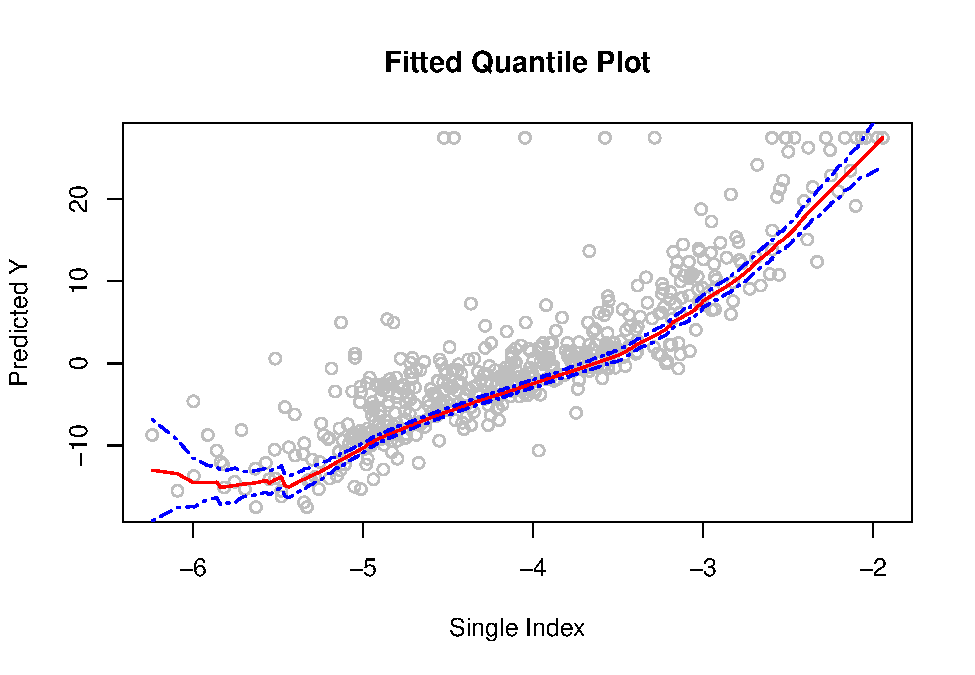
\includegraphics{siqr_files/figure-latex/unnamed-chunk-2-1} \end{Schunk}

\begin{Schunk}
\begin{Sinput}
est.tau50 <- siqr(y0,X,beta.inital = NULL, tau=0.5)
\end{Sinput}
\begin{Soutput}
#> [1] 0
#>         XRM     XlogTAX    XPTRATIO   XlogLSTAT 
#>  0.57091640 -0.36647234 -0.09713939 -0.72822828 
#> [1] 1
#>        xnew1        xnew2        xnew3        xnew4 
#>  0.292809179  0.426155484 -0.005734161  0.855933063 
#> [1] 2
#>       xnew1       xnew2       xnew3       xnew4 
#> 0.009225218 0.372118912 0.026440252 0.927762536 
#> [1] 3
#>       xnew1       xnew2       xnew3       xnew4 
#>  0.12328173 -0.35983254 -0.04707677 -0.92363734 
#> [1] 4
#>       xnew1       xnew2       xnew3       xnew4 
#>  0.22298100 -0.36720391 -0.05962984 -0.90104664 
#> [1] 5
#>      xnew1      xnew2      xnew3      xnew4 
#>  0.2704938 -0.3988501 -0.0634627 -0.8739131 
#> [1] 6
#>       xnew1       xnew2       xnew3       xnew4 
#>  0.28888858 -0.41131208 -0.06460482 -0.86208583 
#> [1] 7
#>       xnew1       xnew2       xnew3       xnew4 
#>  0.30554290 -0.42608004 -0.06319432 -0.84917949 
#> [1] 8
#>       xnew1       xnew2       xnew3       xnew4 
#>  0.30441006 -0.42736713 -0.06305407 -0.84894996 
#> [1] 9
#>       xnew1       xnew2       xnew3       xnew4 
#>  0.30419198 -0.42813835 -0.06305787 -0.84863920 
#> [1] 10
#>       xnew1       xnew2       xnew3       xnew4 
#>  0.30411236 -0.42865435 -0.06304605 -0.84840811 
#> [1] 11
#>       xnew1       xnew2       xnew3       xnew4 
#>  0.30404379 -0.42920321 -0.06303784 -0.84815577 
#> [1] 12
#>       xnew1       xnew2       xnew3       xnew4 
#>  0.30399266 -0.42954021 -0.06302136 -0.84800471
\end{Soutput}
\begin{Sinput}
plot.siqr(est.tau50,bootstrap.interval = TRUE)
\end{Sinput}

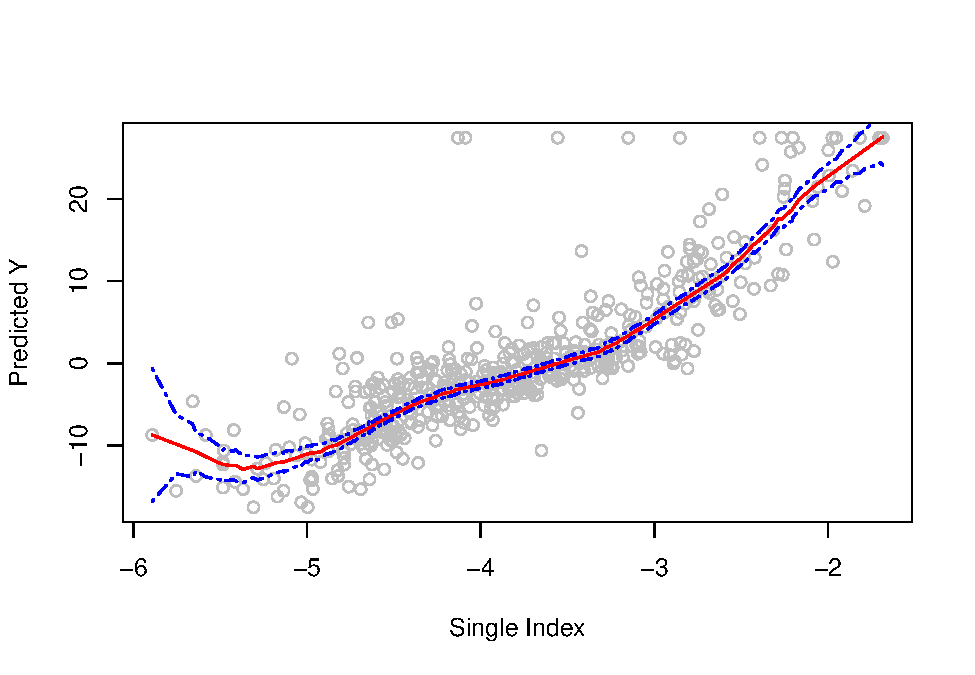
\includegraphics{siqr_files/figure-latex/unnamed-chunk-3-1} \end{Schunk}

\begin{Schunk}
\begin{Sinput}
est.tau75 <- siqr(y0,X,beta.inital = NULL, tau=0.75)
\end{Sinput}
\begin{Soutput}
#> [1] 0
#>         XRM     XlogTAX    XPTRATIO   XlogLSTAT 
#>  0.57054874 -0.10124663 -0.09708887 -0.80919528 
#> [1] 1
#>       xnew1       xnew2       xnew3       xnew4 
#>  0.48765945 -0.15504805 -0.08640925 -0.85479928 
#> [1] 2
#>      xnew1      xnew2      xnew3      xnew4 
#>  0.4437019 -0.1828056 -0.0832210 -0.8733756 
#> [1] 3
#>       xnew1       xnew2       xnew3       xnew4 
#>  0.41422345 -0.18944785 -0.08159574 -0.88649342 
#> [1] 4
#>       xnew1       xnew2       xnew3       xnew4 
#>  0.38561975 -0.19626649 -0.08040366 -0.89794884 
#> [1] 5
#>       xnew1       xnew2       xnew3       xnew4 
#>  0.37307787 -0.19673467 -0.08123174 -0.90305580 
#> [1] 6
#>      xnew1      xnew2      xnew3      xnew4 
#> 0.05565072 0.21650455 0.07029835 0.97215581 
#> [1] 7
#>      xnew1      xnew2      xnew3      xnew4 
#>  0.1319618 -0.2429183 -0.0809211 -0.9576161 
#> [1] 8
#>       xnew1       xnew2       xnew3       xnew4 
#>  0.17237441 -0.23361863 -0.08824924 -0.95284913 
#> [1] 9
#>       xnew1       xnew2       xnew3       xnew4 
#>  0.18360648 -0.22316848 -0.08940544 -0.95314802 
#> [1] 10
#>       xnew1       xnew2       xnew3       xnew4 
#>  0.18835577 -0.21367807 -0.09014301 -0.95432595 
#> [1] 11
#>       xnew1       xnew2       xnew3       xnew4 
#>  0.19350855 -0.20513986 -0.09014037 -0.95516846 
#> [1] 12
#>       xnew1       xnew2       xnew3       xnew4 
#>  0.19532713 -0.19735563 -0.08948809 -0.95649880 
#> [1] 13
#>       xnew1       xnew2       xnew3       xnew4 
#>  0.19600836 -0.19574310 -0.08934566 -0.95670409 
#> [1] 14
#>       xnew1       xnew2       xnew3       xnew4 
#>  0.19621271 -0.19534046 -0.08930334 -0.95674845 
#> [1] 15
#>       xnew1       xnew2       xnew3       xnew4 
#>  0.19646554 -0.19486430 -0.08926289 -0.95679744 
#> [1] 16
#>       xnew1       xnew2       xnew3       xnew4 
#>  0.19674115 -0.19433461 -0.08921794 -0.95685273 
#> [1] 17
#>      xnew1      xnew2      xnew3      xnew4 
#>  0.1968269 -0.1941526 -0.0892026 -0.9568735 
#> [1] 18
#>       xnew1       xnew2       xnew3       xnew4 
#>  0.19686041 -0.19408891 -0.08919724 -0.95688000
\end{Soutput}
\begin{Sinput}
plot.siqr(est.tau75,bootstrap.interval = TRUE)
\end{Sinput}

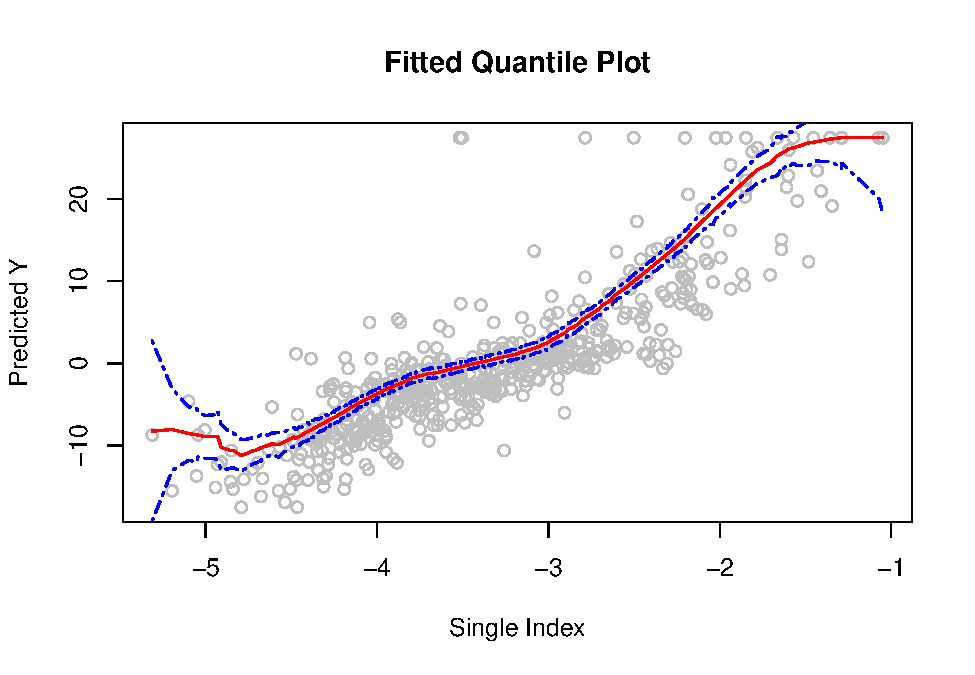
\includegraphics{siqr_files/figure-latex/unnamed-chunk-4-1} \end{Schunk}

\hypertarget{simulation}{%
\subsubsection{Simulation}\label{simulation}}

\hypertarget{setting-1}{%
\paragraph{Setting 1}\label{setting-1}}

\begin{Schunk}
\begin{Sinput}
n <- 400
beta0 <- c(1, 1, 1)/sqrt(3)
n.sim <- 200
tau.vec <- c(0.25,0.5,0.75)
tau <- tau.vec[1]

data <- generate.data(n, true.theta=beta0, setting = "setting1",ncopy = n.sim)

#paralell 
library(parallel)
library(foreach)
cl<- makeCluster(12)
doParallel::registerDoParallel(cl)
sim.results.50 <- foreach(m = 1:n.sim,.combine = "rbind") %dopar% {
  X <- data$X
  Y <- data$Y[[m]]
  est <- siqr(Y, X, beta.inital = c(2,1,0), tau=0.5,maxiter = 30,tol = 1e-8)
  if(est$flag.conv == 0){
    return(NULL)
  }else{
    return(est$beta)
  }
}

sim.results.25 <- foreach(m = 1:n.sim,.combine = "rbind") %dopar% {
  X <- data$X
  Y <- data$Y[[m]]
  est <- siqr(Y, X, beta.inital = c(2,1,0), tau=0.25,maxiter = 30,tol = 1e-8)
  if(est$flag.conv == 0){
    return(NULL)
  }else{
    return(est$beta)
  }
}
sim.results.75 <- foreach(m = 1:n.sim,.combine = "rbind") %dopar% {
  X <- data$X
  Y <- data$Y[[m]]
  est <- siqr(Y, X, beta.inital = c(2,1,0), tau=0.75,maxiter = 30,tol = 1e-8)
  if(est$flag.conv == 0){
    return(NULL)
  }else{
    return(est$beta)
  }
}
stopCluster(cl)
\end{Sinput}
\end{Schunk}

\begin{Schunk}
\begin{Sinput}
sim.results.25 <- readRDS("./sim1.results25.RDS")
sim.results.50 <- readRDS("./sim1.results50.RDS")
sim.results.75 <- readRDS("./sim1.results75.RDS")
\end{Sinput}
\end{Schunk}

\begin{Schunk}
\begin{Sinput}
boxplot(data.frame((sim.results.25)), outline=T,notch=T,range=1,main = "Boxplots of Coefficient Estimates, tau = 0.25",horizontal = F)
\end{Sinput}

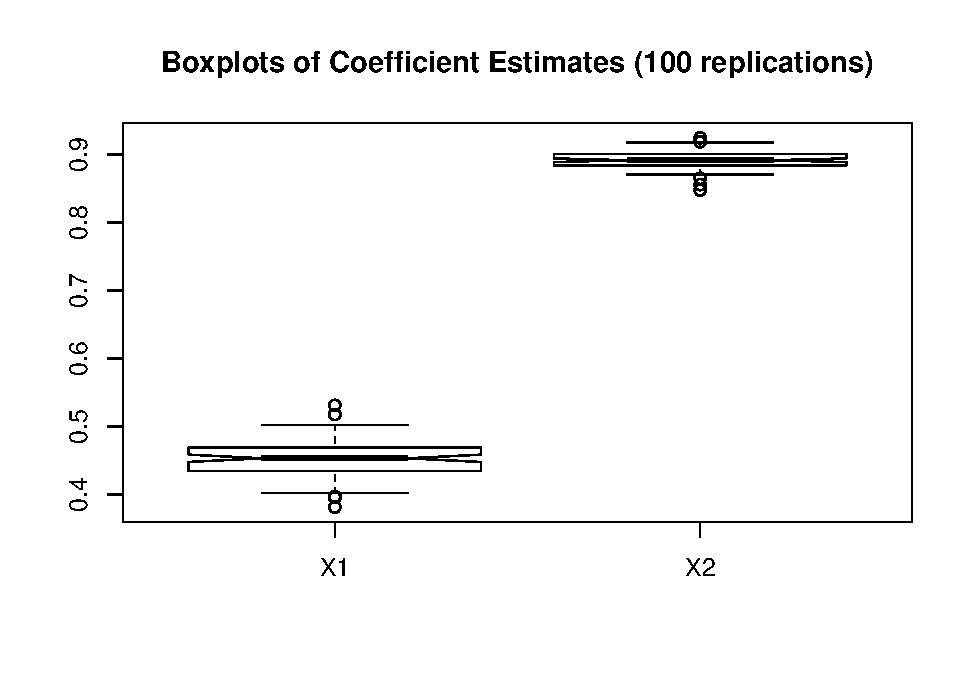
\includegraphics{siqr_files/figure-latex/unnamed-chunk-7-1} \end{Schunk}

\begin{Schunk}
\begin{Sinput}
boxplot(data.frame((sim.results.50)), outline=T,notch=T,range=1,main = "Boxplots of Coefficient , tau = 0.50",horizontal = F)
\end{Sinput}

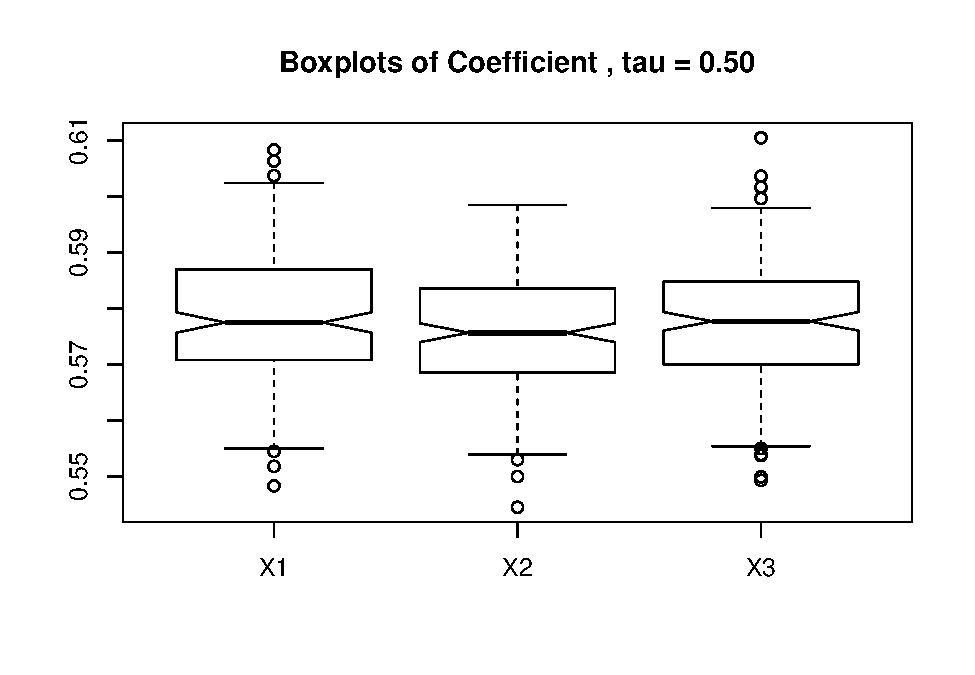
\includegraphics{siqr_files/figure-latex/unnamed-chunk-8-1} \end{Schunk}

\begin{Schunk}
\begin{Sinput}
boxplot(data.frame((sim.results.75)), outline=T,notch=T,range=1,main = "Boxplots of Coefficient Estimates, tau = 0.75",horizontal = F)
\end{Sinput}

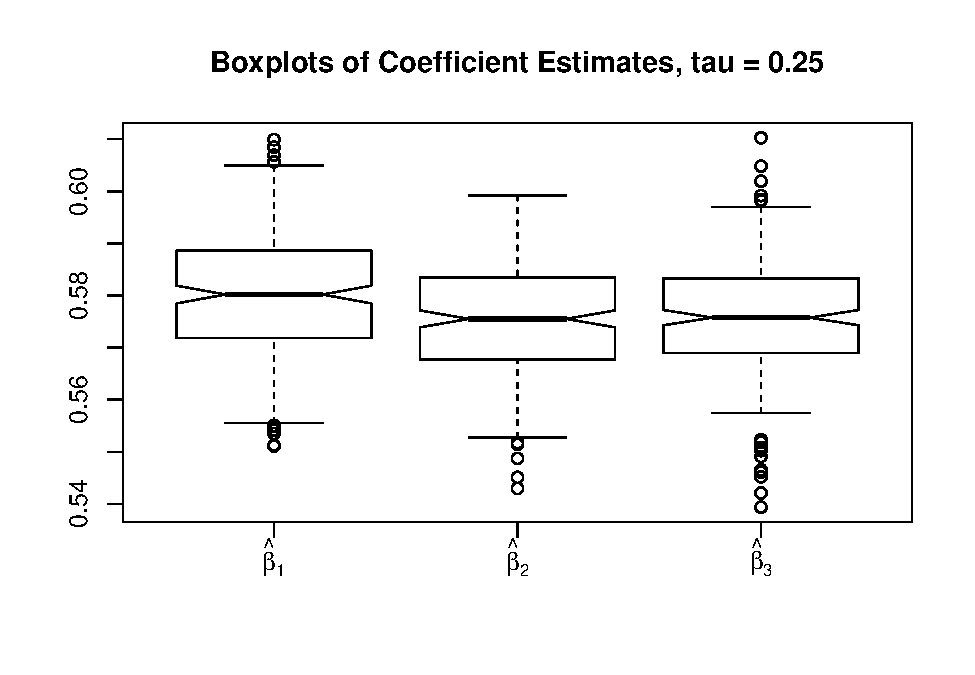
\includegraphics{siqr_files/figure-latex/unnamed-chunk-9-1} \end{Schunk}

\begin{Schunk}
\begin{Sinput}
est.sim.05 <- siqr(data$Y[[1]],data$X,beta.inital = NULL, tau=0.5)
plot.siqr(est.sim.05,bootstrap.interval = TRUE)
\end{Sinput}
\end{Schunk}

\hypertarget{setting-3}{%
\paragraph{Setting 3}\label{setting-3}}

\begin{Schunk}
\begin{Sinput}
n <- 400
beta0 <- c(1, 2)/sqrt(5)
n.sim <- 100
tau <- 0.5

data <- generate.data(n, true.theta=beta0, setting = "setting3",ncopy = n.sim)

#paralell 
library(parallel)
library(foreach)
cl<- makeCluster(12)
doParallel::registerDoParallel(cl)
sim.results <- foreach(m = 1:n.sim,.combine = "rbind") %dopar% {
  X <- data$X
  Y <- data$Y[[m]]
  est <- siqr(Y, X, beta.inital = NULL, tau=tau,maxiter = 30,tol = 1e-8)
  est$beta
}
\end{Sinput}
\end{Schunk}

\begin{Schunk}
\begin{Sinput}
tau <- 0.5
sim.results <- readRDS("./sim.results.RDS")
est.mean <- c(tau,apply(sim.results,2,mean))
names(est.mean) <- c("tau","beta1.hat","beta2.hat")
est.mean
\end{Sinput}
\begin{Soutput}
#>       tau beta1.hat beta2.hat 
#> 0.5000000 0.4515909 0.8917233
\end{Soutput}
\end{Schunk}

\begin{Schunk}
\begin{Sinput}
est.se <- c(tau,apply(sim.results,2,sd))
names(est.se) <- c("tau","beta1.se.hat","beta1.se.hat")
est.se
\end{Sinput}
\begin{Soutput}
#>          tau beta1.se.hat beta1.se.hat 
#>   0.50000000   0.02682211   0.01359602
\end{Soutput}
\end{Schunk}

\begin{Schunk}
\begin{Sinput}
boxplot(data.frame((sim.results)), outline=T,notch=T,range=1,main = "Boxplots of Coefficient Estimates, example 2",horizontal = F)
\end{Sinput}

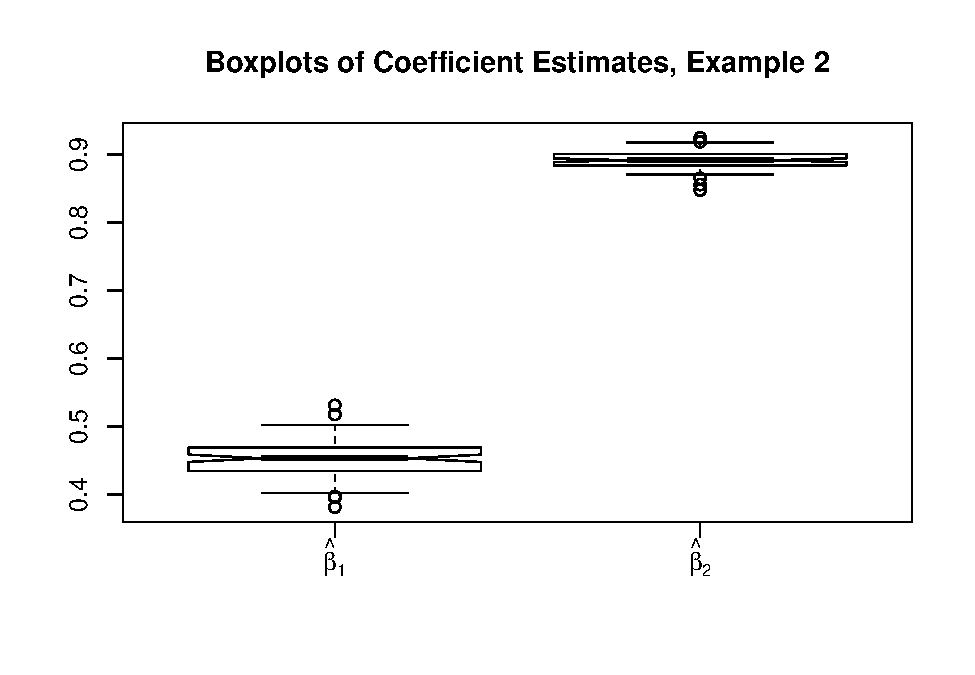
\includegraphics{siqr_files/figure-latex/unnamed-chunk-14-1} \end{Schunk}

\begin{Schunk}
\begin{Sinput}
n <- 400
beta0 <- c(1, 2)/sqrt(5)
n.sim <- 100
tau <- 0.5
data <- generate.data(n, true.theta=beta0, setting = "setting3",ncopy = 2)
est.sim.05 <- siqr(data$Y[[1]],data$X,beta.inital = NULL, tau=0.5)
\end{Sinput}
\begin{Soutput}
#> [1] 0
#>         X1         X2 
#>  0.4591969 -0.8883345 
#> [1] 1
#>      xnew1      xnew2 
#> 0.04819079 0.99883815 
#> [1] 2
#>     xnew1     xnew2 
#> 0.2754254 0.9613224 
#> [1] 3
#>     xnew1     xnew2 
#> 0.3781022 0.9257639 
#> [1] 4
#>     xnew1     xnew2 
#> 0.3986258 0.9171137 
#> [1] 5
#>     xnew1     xnew2 
#> 0.4013716 0.9159153 
#> [1] 6
#>     xnew1     xnew2 
#> 0.4026119 0.9153708 
#> [1] 7
#>     xnew1     xnew2 
#> 0.4034853 0.9149861 
#> [1] 8
#>     xnew1     xnew2 
#> 0.4038987 0.9148037 
#> [1] 9
#>     xnew1     xnew2 
#> 0.4040899 0.9147193 
#> [1] 10
#>     xnew1     xnew2 
#> 0.4042582 0.9146449 
#> [1] 11
#>     xnew1     xnew2 
#> 0.4043899 0.9145867 
#> [1] 12
#>     xnew1     xnew2 
#> 0.4044719 0.9145504 
#> [1] 13
#>     xnew1     xnew2 
#> 0.4045083 0.9145343
\end{Soutput}
\begin{Sinput}
plot.siqr(est.sim.05,bootstrap.interval = TRUE)
\end{Sinput}

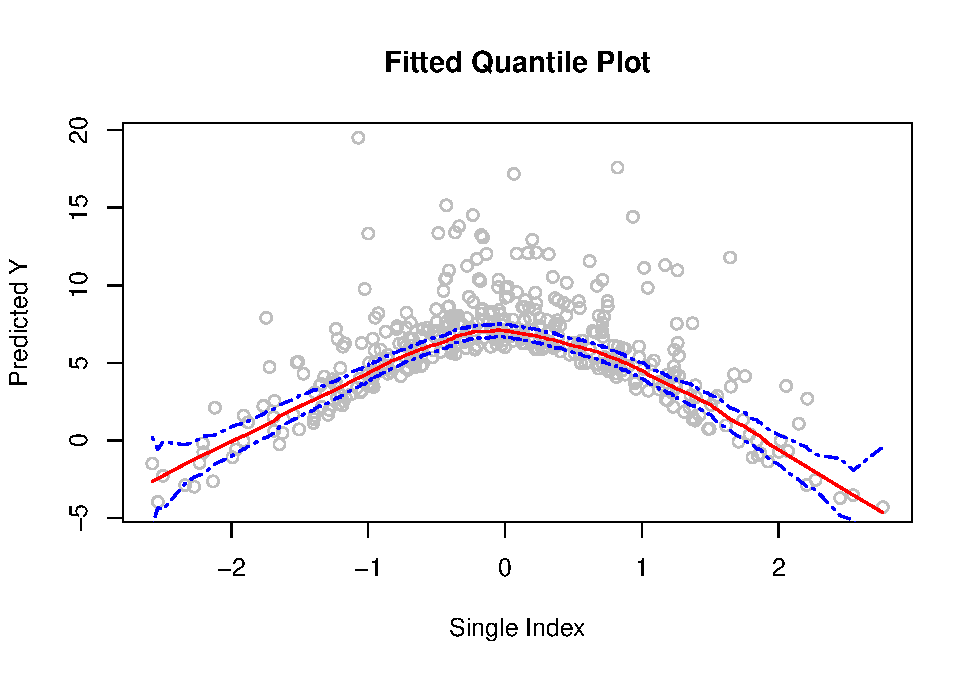
\includegraphics{siqr_files/figure-latex/unnamed-chunk-15-1} \end{Schunk}

\begin{Schunk}
\begin{Sinput}
Sys.sleep(100)
\end{Sinput}
\end{Schunk}

\bibliography{RJreferences}


\address{%
Author One\\
Affiliation\\
line 1\\ line 2\\
}
\href{mailto:author1@work}{\nolinkurl{author1@work}}

\address{%
Author Two\\
Affiliation\\
line 1\\ line 2\\
}
\href{mailto:author2@work}{\nolinkurl{author2@work}}

